\section{Aufbau und Durchführung}
\label{sec:Durchführung}
\begin{figure}
    \centering
    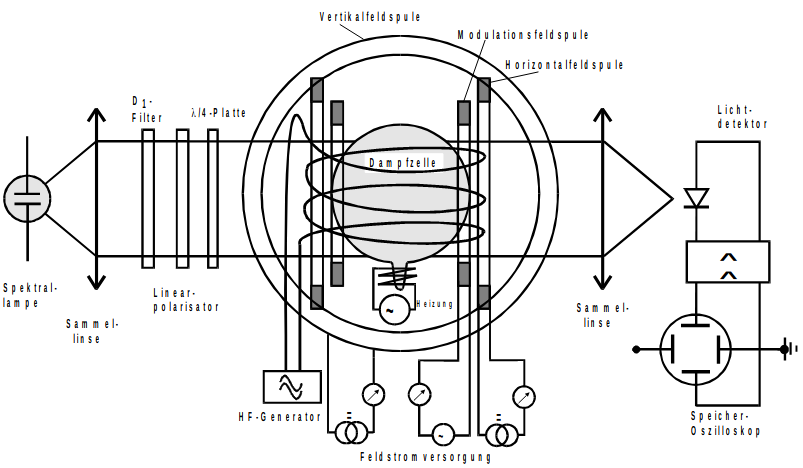
\includegraphics[width = 0.9 \textwidth]{pics/Aufbau.png}
    \caption{Versuchsaufbaut.
    Entmommen aus \cite{sample}}
    \label{fig:Ficken}
\end{figure}
Als Emissionsquelle dient eine Rb-Spektrallampe, die die gebrauchte Wellenlänge für die Übergänge liefert.
Die Sammellinse lässt das Licht parallel verlaufen, um die Verluste zu minimieren.
Fortan filtert der $D_1$-Filter die nicht gebrauchten Wellenlängen raus.
Der lineare Polarisator polarisiert das Licht linear, wonach die $\sfrac{\lambda}{4}$-Platte 
für eine reine rechts-zirkuläre Polarisation des Lichts sorgt, damit die richtigen Auswahlregeln für die Übergänge gelten.
Danach tritt das Licht in drei Magnetfelder von drei Spulen ein. 
Einerseits sorgt ein vertikales Feld für die Kompensation der vertikalen Komponente des Erdmagnetfelds.
Anderseits sind die die beiden horizontalen Spulen, wovon eine Spule eine Sweep-Spule ist, zur Variation der Feldstärke bei verschiedenen 
Frequenzen des HF-Generators, womit die Resonanzen für die induzierte Emission getroffen werden, da.
Die zweite Sammellinse bündelt das Licht, damit eine möglichst hohe Intensität an dem Lichtdetektor ankommt.
Das Signal wird im $x\text{-}y$-Modus am Oszilloskop dargestellt.\\
Als Erstes werden die optischen Geräte so eingestellt, dass die Brennpunkte der Sammellinsen in der Spektrallampe und dem Lichtdetektor liegen und 
eine maximale Intensität an dem Lichtdetektor ersichtlich wird.
Zunächst wird der zur Minimierung der Umwelteinflüsse abgedeckte Aufbau gedreht, so dass die horizontale Feldkomponente der Erde (anti-)parallel zu den horizontalen Feldern 
der Apperatur steht. 
Danach wird die vertikale Komponente des Erdfeldes mittels der vertikalen Spule kompensiert, damit
der Nullpeak möglichst schmal ist.
Nachdem das Erdmagnetfeld berücksichtigt wurde, wird der HF-Generator angeschaltet, womit die $D_1$-Übergänge der beiden Isotope
am Oszilloskop ersichtlich werden.
Die  Frequenzen wurden im Bereich von 100 bis $\qty{1000}{\kilo\hertz}$ in 10 Schritten variiert.
Mittels der Sweep-Spule und der festen horizontalen Spule werden die Peaks gesucht und der Strom, welcher die Magnetfelder beider Spulen induziert, notiert.
